\documentclass[tikz,border=3mm]{standalone}
\usetikzlibrary{arrows.meta}
\usepackage{amssymb}
\begin{document}
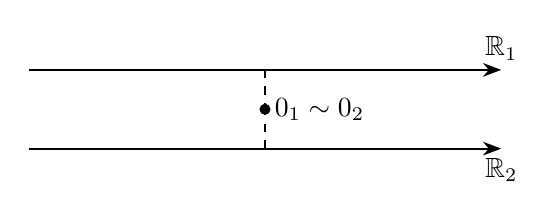
\begin{tikzpicture}[
    line/.style={thick, ->, >=Stealth},
    node distance=2mm
]
    % Прямая ℝ₁ (верхняя линия)
    \draw[line] (-3, 0.5) -- (3, 0.5);
    \node[above] at (3, 0.5) {$\mathbb{R}_1$};
    
    % Прямая ℝ₂ (нижняя линия)
    \draw[line] (-3, -0.5) -- (3, -0.5);
    \node[below] at (3, -0.5) {$\mathbb{R}_2$};
    
    % Точка склейки 0₁ ∼ 0₂
    \fill[black] (0,0) circle (2pt);
    \node[right] at (0,0) {$0_1 \sim 0_2$};
    
    % Пунктирные линии, соединяющие нули с общей точкой
    \draw[dashed] (0, 0.5) -- (0,0);
    \draw[dashed] (0, -0.5) -- (0,0);
\end{tikzpicture}
\end{document}